% !TEX output_directory = ./build

\documentclass[master,english]{hgbthesis}
% Zulässige Class Options:
%   Typ der Arbeit: diplom, master (default), bachelor, praktikum
%   Hauptsprache: german (default), english
%%------------------------------------------------------------

\graphicspath{{images/}}    % wo liegen die Bilder?
\bibliography{library}  	% Angabe der BibTeX-Datei, % utf8-change

\usepackage{tikz}
\usepackage{subfigure}
\usepackage{pgfplots}
\usepackage{amsmath}
\usepackage{amsmath,amssymb}
\usepackage{mathtools}
\usepackage[algo2e]{algorithm2e}
\usepackage[top=3cm,left=3cm,right=3cm,bottom=3cm]{geometry}
% Scriptsize axis style.
\usepackage{bookmark}
\pgfplotsset{every axis/.append style={tick label style={/pgf/number format/fixed},font=\scriptsize,ylabel near ticks,xlabel near ticks,grid=major}}

\usetikzlibrary{matrix,chains,positioning,decorations.pathreplacing,arrows}


\DeclareMathOperator*{\argmin}{argmin}
\DeclareMathOperator{\E}{\mathbb{E}}
\DeclarePairedDelimiter{\ceil}{\lceil}{\rceil}

%%%----------------------------------------------------------
\begin{document}
%%%----------------------------------------------------------

% Einträge für ALLE Arbeiten: --------------------------------
\title{Solving localization problem in first person computer games with deep learning}
\author{Yauheni\ Selivonchyk}
\studiengang{Computer Science}
\studienort{Rheinische Friedrich-Wilhelms-Universität Bonn}
\abgabedatum{2017}{03}{30}	% {YYYY}{MM}{DD}

%%% zusätzlich für eine Bachelorarbeit: ---------------------
\nummer{XXXXXXXXXX-A}   % XX...X = Stud-ID, z.B. 0310238045-A
                        % (A = 1. Bachelorarbeit)
\semester{Sommersemester 2017}
\gegenstand{Einführung in die Tiefere Problematik 1}
\betreuer{Prof. Dr. Christian Bauckhage Alois} % oder \betreuerin{..}

%%% zusätzlich für einen Praktikumsbericht: -----------------
\nummer{XXXXXXXXXX-B}   % XX...X = Stud-ID, z.B. 0310238045-B
                        % (B = 2. Bachelorarbeit)
\betreuer{Mag.~Pjotr I.~Czar\\Creative Director}  % \betreuerin{..}
\firma{%
   Oligarchic Media International GmbH\\
   Online Division\\
   1020 Wien, Hubertusgasse 3a
}
\firmenTel{1-234-5678-100}
\firmenUrl{www.mogul.at}

%\strictlicense  % erzeugt restriktive Lizenzformel

%%%----------------------------------------------------------
\frontmatter
\maketitle
\tableofcontents
%%%----------------------------------------------------------

% \include{vorwort}		% ggfs. weglassen
% \include{kurzfassung}
\chapter{Abstract}

\begin{english} %switch to English language rules
This should be a 1-page (maximum) summary of your work in English.
%und hier geht dann das Abstract weiter...
\end{english}

Im englischen Abstract sollte inhaltlich das Gleiche
stehen wie in der deutschen Kurzfassung. Versuchen Sie daher, die
Kurzfassung prä\-zise umzusetzen, ohne aber dabei Wort für Wort zu
übersetzen. Beachten Sie bei der Übersetzung, dass gewisse
Redewendungen aus dem Deutschen im Englischen kein Pendant haben
oder völlig anders formuliert werden müssen und dass die
Satzstellung im Englischen sich (bekanntlich) vom Deutschen stark
unterscheidet (mehr dazu in Abschn.\ \ref{sec:englisch}). Es
empfiehlt sich übrigens -- auch bei höchstem Vertrauen in die
persönlichen Englischkenntnisse -- eine kundige Person für das
"`proof reading"' zu engagieren.

Die richtige Übersetzung für "`Diplomarbeit"' ist übrigens
schlicht \emph{thesis}, allenfalls  "`diploma thesis"' oder "`Master's thesis"', 
auf keinen Fall aber "`diploma work"' oder gar "`dissertation"'. 
Für "`Bachelorarbeit"' ist wohl "`Bachelor thesis"' die passende Übersetzung. 

Übrigens sollte für diesen Abschnitt die \emph{Spracheinstellung} in \latex\ von Deutsch
auf Englisch umgeschaltet werden, um die richtige Form der
Silbentrennung zu erhalten, die richtigen Anführungszeichen muss
man allerdings selbst setzen %
(s.\ dazu die Abschn.\ \ref{sec:sprachumschaltung} %
und \ref{sec:anfuehrungszeichen}).


%%%----------------------------------------------------------
\mainmatter         % Hauptteil (ab hier arab. Seitenzahlen)
%%%----------------------------------------------------------

% !TEX root = ./thesis.tex

\chapter{Introduction}
\label{ch:intro}

Learning Deep Architectures for AI \cite{Bengio2009}




%Das geht dann so \cite{Lamport95}.

% !TEX root = ./thesis.tex

\chapter{Related work}
\label{ch:rewo}
Stacked conv AE \cite{Masci2011} introduce Convolutional Auto-Encoder for hierarchical feature extraction.
They claim, that initializing CNN with convolutional layers of trained CAE consistently increases perfromance of a CNN.

VAE. Tutorial on VAE \cite{Doersch2016}

Rationalizing Neural Prediction \cite{Lei2016}


\textit{recommended by tutors}
NG Sparse AE  \cite{Ng2011} introduces notion of sparcity properly
Learning Deep Architectures for AI \cite{Bengio2009}
Stacked convolutional auto-encoders for hierarchical feature extraction \cite{Masci2011}

Spatial Transformer Networks \cite{Jaderberg2015}

Loop closure detection for visual SLAM systems using deep neural networks \cite{Gao2015}
Authors build a denoising autoencoder with sparce objective adding continuity objective.
Continuity objective enforces L2 similaraty between extracted features for consequtive frames. They use dataset: freiburg2 slam.
Deep Convolutional Inverse Graphics Network \cite{Kulkarni2015}.
Based on idea of VAE XXX build a network that extracts features related to spatial transformations of 3D objects.

Understanding Visual Concepts with Continuation Learning \cite{Whitney2016}
Authors propose a neural network archtecture for extracting a subset of highly interpretable features
from image sequencies.

Stacked Denoising Autoencoders: Learning Useful Representations in a Deep Network with a Local Denoising Criterion \cite{Vincent2010}

Loop closure:
Loop Closure Detection for Visual SLAM Using PCANet Features.
Unsupervised learning to detect loops using deep neural networks for visual SLAM system.
VLAD-Based Loop Closure Detection For Monocular SLAM.
\cite{Xia2016, Gao2015a, Huang2016}



Autoencoders

Stacked What-Where Auto-encoders \cite{Zhao2015}
Auto-Encoding Variational Bayes \cite{Kingma2013}

Deep Learning \cite{LeCun2015}

Notion of sparcity


Localization issues

% !TEX root = ./thesis.tex

\chapter{Technical details}
\label{ch:tede}

This chapter provides technical details relevant to the method proposed in chapter \ref{ch:mode}.
In subsection \ref{ch:nn} we provide overview of artificial neural networks and related optimization techniques.
Subsection \ref{ch:ae} describes several unsupervised learning techniques for artificial neural networks also known as autoencoders.

\section{Artificial Neural Networks}
\label{ch:nn}
An artificaial neural network is a methematical model that loosly resembling biological brain structure.

An artificial neural network is a mathematical model inspired by biological brain structure.
A neural network comprises of a set of interacting computational units, called neurons.
In practise, neurons' computation contains a linear transformation of inputs followed by an activation function.
Sigmoid, ReLU and identity functions are among most commonly used activation function.

Neural networks are organized in layers.
A layer can be viewed as a set of neurons that rely on same inputs and have similar behaviour i.e. activation function, output size, regularization parameters.
We also distinguish auxilary layers that perform some transformation of the input data.
Scaling layer, applying non-liniarity function and pooling layer are one of many examples of such layes.

Major neural networks groups are distinguished between each other by structure of connections between neurons.
Feedforward neural networks prohibit cyclic connection and loops in network structure, while Recurent neural networks have no such restiction.

In subsection \ref{ch:ffnn} we are going to describe basic building blocks of feedforward neural network.
Subsection \ref{ch:cnn} describes of a special case of feedforward neural network with parameter sharing.
Finally, in subsection \ref{ch:opt} we deiscuss basis concepts of training artificial neural networks.

% \subsection{Artificial Neural Network}
\subsection{Feedforward Neural Networks}
\label{ch:ffnn}

Perceptron is a simplest example of single layer artificial neural network.
Performs linear combination of input values $x$ and some constant value $b$ called \textit{bias} and applies some activation function $f$ to produce output:
\begin{equation}\label{eq:per}
  y = f(\sum_{i=1}^N W_ix_i + b) = f(Wx+b)
\end{equation}
where $W$ is a column vector of perceptron parameters and $f$ is an activation function. Structure of perceptron is depicted on figure \ref{fig:perc}.

% !TEX root = ../thesis.tex

\begin{figure}

\centering
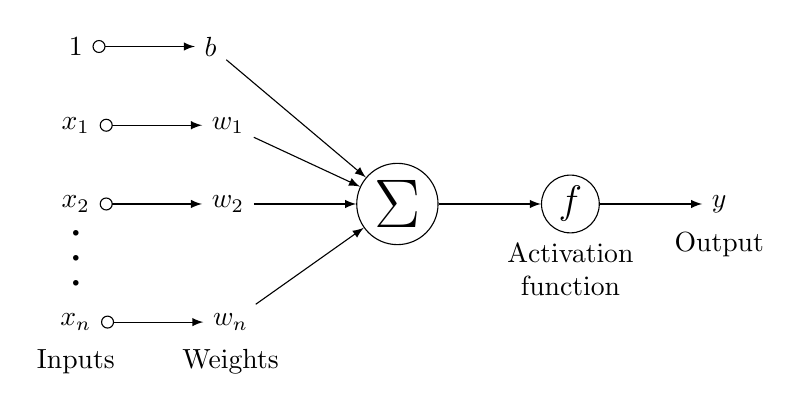
\begin{tikzpicture}[
init/.style={
  draw,
  circle,
  inner sep=2pt,
  font=\Huge,
  join = by -latex
},
act/.style={
  draw,
  circle,
  inner sep=2pt,
  font=\Large,
  join = by -latex
},
squa/.style={
  draw,
  inner sep=2pt,
  font=\Large,
  join = by -latex
},
start chain=2,node distance=13mm
]
\node[on chain=2]
  (x2) {$x_2$};
\node[on chain=2,join=by o-latex]
  {$w_2$};
\node[on chain=2,init] (sigma)
  {$\displaystyle\Sigma$};
\node[on chain=2,act,label=below:{\parbox{2cm}{\centering Activation \\ function}}]
  {$f$};
\node[on chain=2,label=below:Output,join=by -latex]
  {$y$};
    % {[shift={(0.0,-2.0)}]\centering Activation \\ function}

\begin{scope}[start chain=4]
\node[on chain=4] at (0,2.0cm)
  (b) {$ 1$};
\node[on chain=4,join=by o-latex]
  (w0) {$b$};
\end{scope}

\begin{scope}[start chain=1]
\node[on chain=1] at (0,1.0cm)
  (x1) {$x_1$};
\node[on chain=1,join=by o-latex]
  (w1) {$w_1$};
\end{scope}

\begin{scope}[start chain=3]
\node[on chain=3,label=below:Inputs] at (0,-1.5cm)
  (x3) {$x_n$};
\node[on chain=3,label=below:Weights,join=by o-latex]
  (w3) {$w_n$};
\end{scope}
% \node[label=above:\parbox{2cm}{\centering Bias \\ $b$}] at (sigma|-w1) (b) {};

\draw[-latex] (w0) -- (sigma);
\draw[-latex] (w1) -- (sigma);
\draw[-latex] (w3) -- (sigma);
% \draw[o-latex] (b) -- (sigma);

% \draw[decorate,decoration={brace,mirror}] (x1.north west) -- node[left=10pt] {Inputs} (x3.south west);
% \draw[decorate,decoration={brace,mirror}] (b.north west) -- node[left=10pt] {Bias} (b.south west);
\path (x2) -- (x3) node [font=\huge, midway, sloped] {$\dots$};
\end{tikzpicture}
\caption{Single layer neural network (perceptron) calculates some function on linear combination of its inputs according to the set of weights $W$.  }
\label{fig:perc}
\end{figure}


By combining several perceptrons in one set we can produce multiple output values of $y$.
For simplicity, we will stack parameters of $j$ multiple perceptrons that use the same input size $i$ into matrixes $W$ and $b$, where $W$ is rectrangular matrix of size $[i,j]$ and $b$ is a column vector of size $j$.
In this case equation $\ref{eq:per}$ remains the same for column vector $y$ of size $j$. Set of perceptron-like neurons that perform computation on same input forms a single \textit{fully connected} layer of multilayer neural network.

When we combine several layers together we would refer to inut vector $x$ as to \textit{input layer} and to last layer of the network producing final output $y$ as \textit{output layer}. All intermidiate layers between input and output are called \textit{hidden layers}.

It has been shown, that artificial neural network under mild assumption about form of activation function can act as universal approximator even using single layer of hidden units of finite size \cite{Debao1993}.
Even though single hidden layer must be enough for a large family of functions, it might take exponentially many units to performs such approximation \cite{Pascanu2014}.
Hence, many researchers are developing neural networs with hundreeds of layers to allow more compact representation of complex functions \cite{He2015, Srivastava2015}.

Expressivity of the functions that can be approximated by a neural network comes at a cost.
Extensively complex models are prone to overfitting. Overfitting occuars when model learns from unimportant latent concepts in the input data.
In other words, overlycomplex model is likely to learn distribution of noise in the input data instead of a useful concept.
Overfitting leads to misleadingly high performance of the model on the training set but signifficantly lower solution qualities on yet unseen data.

Collecting more data, regularizing the model and decreasing the complexity of the model are groups of techniques that allow to fight the overfitting.


% !TEX root = ../thesis.tex

\begin{figure}[t!]
	\centering
	\subfigure[Logistic sigmoid.]{
    		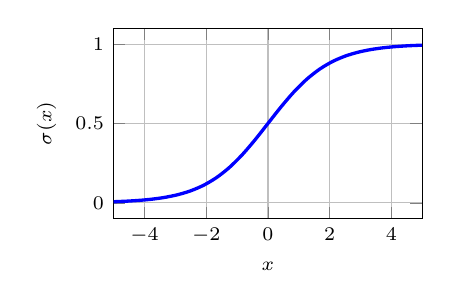
\begin{tikzpicture}
			\begin{axis}[width=5.5cm,height=4cm,ylabel=$\sigma(x)$,xlabel=$x$,ymin=-0.1,ymax=1.1,xmin=-5,xmax=5]
				\addplot[very thick,blue,smooth] {1/(1+exp(-x))};
			\end{axis}
		\end{tikzpicture}
	}
	\subfigure[Hyperbolic tangent.]{
		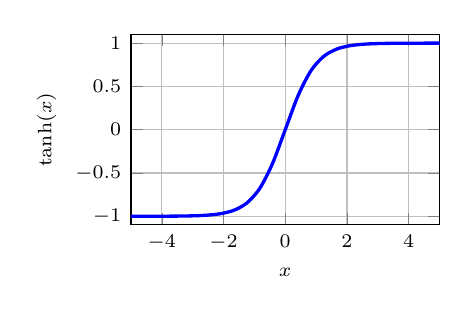
\begin{tikzpicture}
			\begin{axis}[width=5.5cm,height=4cm,ylabel=$\tanh(x)$,xlabel=$x$,ymin=-1.1,ymax=1.1,xmin=-5,xmax=5]
				\addplot[very thick,blue,smooth] {tanh(x)};
			\end{axis}
		\end{tikzpicture}
	}\\
	\subfigure[Rectifier linear unit.]{
    		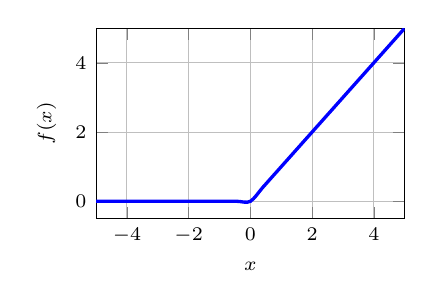
\begin{tikzpicture}
			\begin{axis}[width=5.5cm,height=4cm,ylabel=$f(x)$,xlabel=$x$,ymin=-0.5,ymax=5,xmin=-5,xmax=5]
				\addplot[very thick,blue,smooth] {max(0, x)};
			\end{axis}
		\end{tikzpicture}
	}
	\subfigure[Identity function.]{
		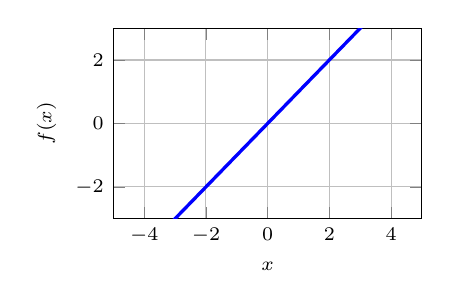
\begin{tikzpicture}
			\begin{axis}[width=5.5cm,height=4cm,ylabel=$f(x)$,xlabel=$x$,ymin=-3,ymax=3,xmin=-5,xmax=5]
				\addplot[very thick,blue,smooth] {x};
			\end{axis}
		\end{tikzpicture}
	}
    	\caption[Sigmoidal activation functions.]{Common choise of activation functions includes logistic sigmoid $\sigma(z)$ and hyperbolic tangent $tanh(z)$. Convolutional neural networks often rely on ReLU and identity functions.}
    	\label{fig:act}
\end{figure}


% \subsection{Artificial Neural Network}
\subsection{Convolutional Neural Networks}
\label{ch:cnn}

Convolutional neural network is a special kind of feedforward neural network that takes advantage of structural organization of the data. This technique allows to decrease number of parameters of the model when applied to structured data.

Many types of data contain redundant information .i.e. information that, when ignored, can be recovered from the remaining data.
For instance, we can rather easily reconstruct skipped word in the sentence "Clouds are in the \_\_" as well as we can recognize an object on an image even if some pixels are altered or missing.
In other words, components of textual or visual data are highly spacially correlated.

Convulutional neural network uses small spacially adjascent parts of data as an input to computational unit. Additionally, computational units that are applied to different pathces can use same set of parameters $K$ called \textit{convoutional kernel} to reduce complexity of the model. A computational unit depending on some kernel $K$ is called a \textit{convolutional filter}. A set of output produced by a single convolutional filter is called a \textit{feature map}.



For an image $I$ of size $H \times W \times C$, where $H$,$W$,$C$ are width, height and number of color channels correspondingly, applying convolutional filter $K$ of size $w \times h$ would result in a feature map of size $(H-h+1) \times (W-w+1) \times 1$. Convolution operation can be described as:
\begin{equation}\label{eq:conv}
  (I \cdot K)_{x, y} = \sum_a \sum_b K_{a,b} I_{x+a, y+b}
\end{equation}
where ${x, y}$ and ${a,b}$ are two-dimensional indexes of feature map and convolution correspondingly and next constrains apply
\begin{equation*}
  \begin{aligned}
  &1 \leq  x \leq H-h+1, \\
  &1 \leq  y \leq W-w+1, \\
  &1 \leq  a \leq h, \\
  &1 \leq  b \leq w
\end{aligned}
\end{equation*}

\begin{figure}
  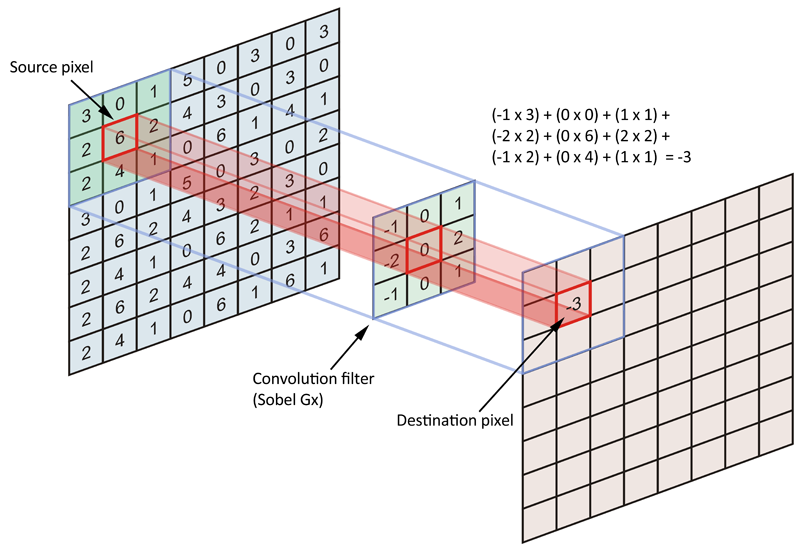
\includegraphics[width=\textwidth,height=\textheight,keepaspectratio]{cnn.png}
  \caption{Illustration of applying convolutional filter of size 3x3 to a single square patch. Output feature map is padded to preserve same shape as input data. Picture taken from [community.arm.com]}
  \label{fig:cnn}
\end{figure}

In convolutional layer output of operation \ref{eq:conv} is used with additional bias $b$.
Sum $(I \cdot K)_{x, y}+b$ is called \texttt{preactivation} and is forwarded to activation function $f$.

\subsubsection{Max-pooling layer}

Pooling layers effectivey reduce size of activation map.


\subsection{Parameter learning}
\label{ch:opt}

TODO: rework with empirical risk minimization in mind. introduce notioin of generalization error

Even though a multilayer neural network can approximate large family of compact functions arbitrary well \cite{Debao1993}, finding the right parameters for such approximation is non-trivial.
Lets consider some error function $L(y, f(x, \theta))$ that calculates error between expected values $y$ and output of the function $f$, realized by a neural network depending on parameters $\theta$. Finding the solution for general neural network is equivalent to solving next optimization problem:

\begin{equation}\label{eq:optnn}
  \hat{\theta} = J(\theta) = \argmin_{\theta \in \Bbb{R}^D} \frac{1}{N} \sum_{i=1}^{N} L(y_i, f(x_i, \theta))
\end{equation}
where $D$ is equivalent to number of parameters $||\theta||$ and $N$ is the size of the training set.

Problem \ref{eq:optnn} in general case has no closed-form solution and finding optimal set of parameters $\hat{\theta}$ is an NP-hard problem \cite{Anandkumar16}.
In practise, gradient descent methods are used to find good parametrization $\hat{\theta}$ of the neural network.

Gradient descent methods suggests to iteratively update parameters $\theta_t$ each time taking a step $\eta$ towards the direction of a better solution $\theta_{t+1}=\theta_t - \eta \nabla_\theta \theta$ \cite{Cauchy1847}.
We use vector partial derivatives $\nabla_\theta J(\theta)=\{ \frac{\partial J(\theta)}{\partial w_1}, \ldots, \frac{\partial J(\theta)}{\partial w_N} \}$ of function $J(\theta)$ at point $\theta_t$ as the the direction towards better solution. Gradient descent method requires both funcitons $L(y, \hat{y})$ and $f(x, \theta)$ to be differentiable. Note, that differentiablility of function $f(x, \theta)$ in $\theta$ implies differentiability of the activation fucntion \ref{eq:per}. Algorithm pseudocode is shown on listing \ref{alg:bp}.

% !TEX root = ../thesis.tex

\begin{algorithm}[H]
 \KwData{X, Y  \text{ (Train set)}}
 \KwResult{$\theta \text{ (Learned weights)}$}

 ${\textbf{Require: } \eta\text{: Stepsize}}$

 $\theta \gets \theta_0 \text{ (Initialization)}$

 \While{not time to terminate}{
  $\triangle_\theta \gets \nabla_\theta J(\theta)(X, Y) \text{ (Calculate gradients)}$

  $\theta \gets \theta - \eta \triangle_\theta\text{ (Update weights)}$

 }

 \Return $\theta$

 \caption{Gradient descent algorithm}\label{alg:bp}

\end{algorithm}


Gradient based methods do not guarantee to find the optimal solution.
Traing can stop in a local minima ($\theta \leq \theta + \eta \delta | \forall \delta \text{ s.t. } |\delta|^2 \leq \epsilon$) or a saddle point.
These cases are shown on figure \ref{fig:critical}.

\begin{figure}[h!]
  \centering
    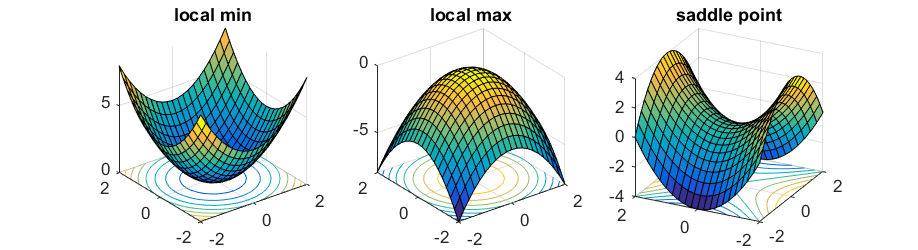
\includegraphics[width=\textwidth,height=\textheight,keepaspectratio]{minmaxsaddle.png}
  \caption{Critical points of a loss fucntion $f(x)$, where $x \in \Bbb{R}^2$.}
  \label{fig:critical}
\end{figure}

In practise, solutions produced by gradient based methods has proven to have suttisfying qualities \cite{Szegedy2016,He2015}.
This might be due to the properties of high-dimensional non-convex error surfaces. The study by Y.Dauphin et al. \cite{Dauphin14} concludes, that saddle points and local minima on such surfaces are very likely to be close to the global minima.

\subsubsection{Stochastic gradient descent with minibatches}

Algorithm \ref{alg:bp} requires full path through the complete training data on each iteration.
This might be computationally wasteful for large datasets. Instead, we can perform optimization iteratively only considering subsets of the traingin set, drawn i.d.d. from the training set:

\begin{equation*}\label{eq:sopt}
  \begin{aligned}
  & \frac{1}{N} \sum_{i=1}^{N} L(y_i, f(x_i, \theta)) = \E_{i \sim U(1,N) } L(y_i, f(x_i, \theta)) \\
  & \E_{i \sim U(1,N) } L(y_i, f(x_i, \theta))= \frac{1}{M} \E_{m \sim U^M(1,N) } \sum_{i \in m} L(y_i, f(x_i, \theta))
  \end{aligned}
\end{equation*}

As a resutl, we can use stochastic procedure of selecting $M$ inputs from training dataset to use in each training iteration.
Subset of inputs selected this way are called \textbf{minibatches}. Updated algorithm is shown on listing \ref{alg:sbp}.

% !TEX root = ../thesis.tex

\begin{algorithm}[H]
 \KwData{X, Y  \text{ (Train set)}}
 \KwResult{$\theta \text{ (Learned weights)}$}

 \Require{\textbf{Require: } \eta\text{: Stepsize}}

 \Require{\textbf{Require: } \M\text{: Minibatch size}}

 \State \theta \gets \theta_0 \text{ (Initialization)}

 \While{not time to terminate}{
  \State X_i, Y_i \gets \text{Select $M$ examples i.i.d. from $X, Y$}

  \State \triangle_\theta \gets \nabla_\theta J(\theta)(X_i, Y_i) \text{ (Calculate gradients)}

  \State \theta \gets \theta - \eta \triangle_\theta\text{ (Update weights)}

 }

 \Return{\theta}

 \caption{Stochastic gradient descent algorithm with minibatches}\label{alg:sbp}

\end{algorithm}


\subsubsection{Adam update rule}

Training time of gradient descent based algorithm can be reduced by applying adaptive learning rates \cite{Kingma2015}.
\textit{Adam update rule} or simply Adam is one of the algorithm that allow to reduce training time of gradient descent.

Adam update rule maintains exponential moving average of the gradients $m_t$ and the squared gradient $v_t$.
Hyperparameters $\beta_1, \beta_2$ set the exponential decay rates for both sets of variables.
Update rule for exponential moving average is as follows:
\begin{equation*}
  \begin{aligned}
    & m_t = \beta_1 \cdot m_{t-1} + (1-\beta_1) \cdot g_t \\
    & v_t = \beta_2 \cdot v_{t-1} + (1-\beta_2) \cdot g_t^2
  \end{aligned}
\end{equation*}

Variables $m_t$ and $v_t$ are estimating 1st and 2nd moments of the gradients.
We can therefore rewrite update rule:
\begin{equation}
  \theta_t \gets \theta_{t-1} - \eta m_t / (\sqrt{v_t} + \epsilon)
\end{equation}
where $\epsilon$ is a small guard value that prevents divisor from getting to close to zero.

Exponential moving averages $m_t$ and $v_t$ are initialized with zeros.
This leads to zero-bias of the estimators during initial phase of the trainging.
To accelerate learning process during first iterations of algorithm \ref{alg:sbp} a time dependent regularization is applied:
\begin{equation*}
  \begin{aligned}
    & \hat{m} = m / (1-\beta_1^t) \\
    & \hat{v} = v/(1-\beta_2^t)
  \end{aligned}
\end{equation*}
where $t$ is a variable tracking current iteration number.

Algorithm requires memory overhead proportinal to the number of parameters $||\theta||$. Listing \ref{alg:adam} shows the full algorithm of Adam update rule written in pseudocode.

% !TEX root = ../thesis.tex

\begin{algorithm}[H]
	\KwData{X, Y  \text{ (Train set)}}
	\KwResult{$\theta \text{ (Learned weights)}$}

	$\textbf{Require: } \eta\text{: Stepsize}$

	$\textbf{Require: } \beta_1, \beta_2 \in [0, 1) \text{: Exponential decay rates for the moment estimates}$

	$\textbf{Require: } f(\theta) \text{: Stochastic objective function with parameters } \theta$

	$\textbf{Require: } \theta_0 \text{: Initial parameter vector}$

	$m_0 \gets 0 \text{ (Initialize 1st moment vector)}$

	$v_0 \gets 0 \text{ (Initialize 2nd moment vector)}$

	$t \gets 0 \text{ (Initialize timestep)}$

	\While {$\theta_t$ not converged}{

		$t \gets t + 1$

		$g_t \gets \nabla_\theta f_t(\theta_{t-1}) \text{ (Get gradients w.r.t. stochastic objective at timestep t)}$

		$m_t \gets \beta_1 \cdot m_{t-1} + (1-\beta_1) \cdot g_t \text{ (Update biased first moment estimate)}$

		$v_t \gets \beta_2 \cdot v_{t-1} + (1-\beta_2) \cdot g_t^2 \text{ (Update biased second raw moment estimate)}$

		$\hat{m}_t \gets m_t / (1-\beta_1^t) \text{ (Compute bias-corrected first moment estimate)}$

		$\hat{v}_t \gets v_t/(1-\beta_2^t) \text{ (Compute bias-corrected second raw moment estimate)}$

		$\theta_t \gets \theta_{t-1} - \eta \cdot \hat{m}_t / (\sqrt{\hat{v}_t}+\epsilon) \text{ (Update parameters)}$
	}
	$\textbf{return: } \theta_t \text{ (Resulting parameters)}$

	\caption{Adam, stochastic optimization algorithm. Default settings that work good for tested problems $\eta=0.0001 \ldots 0.001$, $\beta_1=0.9$, $\beta_2=0.999$ and $\epsilon=10^{-8}$} \label{alg:adam}

\end{algorithm}


\subsection{Regularization}
\subsubsection{Dropout}
\subsubsection{Data augmentation}





\section{Autoencoders}\label{ch:ae}
An autoencoder or autoassociator neural network is an unsupervised learning algorithm that sets target output values equal to input values $y_i=x_i$ \cite{Ng2011,RanzatoMarcAurelio2007}.
Autoencoders are usually trained according to \textit{encoder-decoder} paradigm.
Which first allows to project or encode input $x_i$ into some useful feature representation $h_i$.
Then reconstruct or decode original input $\hat{y_i}$ from representation $h_i$.
This process is schematically on image \ref{fig:ae}.

\begin{figure}[h!]
  \centering
    
\includegraphics[width=\textwidth,height=\textheight,keepaspectratio]{ae.png}
  \caption{Autoencoder.}
  \label{fig:ae}
\end{figure}



We are going to refer to encoder as a deterministic differentiable function $f(x, \theta_f)$ that for a given set of parameters $\theta_f$ maps input $x\in \Bbb{R}^d$ into representation $h \in \Bbb{R}^{d'}$.
Likewise, decoder is deterministic differentiable function $g(h, \theta_g)$ depending on parameters $\theta_g$ maps $h\in\Bbb{R}^{d'}$ into $y\in \Bbb{R}^d$. We will further avoid specifying parameters $\theta_f$ and $\theta_g$ for simplicity.
Given a loss function $L$, for a dataset $X=\{x_0, ..., x_i\}$ we can define learning objective as follows \cite{Good2016}:

\begin{equation}\label{eq:ae}
\min_{\theta_f, \theta_g}\sum\limits_{x_i \in X}{L(x_i, g(f(x))}
\end{equation}

Learning identity mapping itself is not particularly useful.
Instead we are often interested in reusing only parts of the autoencoder.
For example, parameters of the encoder $\theta_f$ can serce as a good initialization of a dicriminative model \cite{Masci2011, Vincent2010, Zhao2015}.
Such initialization results in minor yet coherent improvement of generalization properties of the model.
Variational Autoencoders, on the other hand, reuse decoder as a generator of new training examples \cite{Kingma2013}.
Extracted features $h$ can represent interpretable properties of the input and can be used to adjust this
properties during generation process \cite{Kulkarni2015, Whitney2016}.

Learning useful feature representation is not a trivial task.
One of the common issues with training autoencoders is possibility to learn identity mapping of input data.
Learning identity mapping would result in less informative feature representation of the inputs.
For example, we can represent both encoder and decoder as a linear function and set the size of the feature space so that it exceeds the size of input space $d' > d$.
Then components of autoencoder can both learn simple identity mapping from input space into feature space and wise-versa.
Therefore, it is common to either limit capacity of the feature space to be less than input space or impose additional regularization on extracted features.

Additionally, both encoder and decoder can be represented as arbitrary neural network.
If capacity of any of two networks is hight enough, it would again lead to learning of identity mapping.
On the other hand, if capacity is chosen too low it can hurt the learning process.
For example, low capacity of generator network in Variational Autoecoders can result in mode collapse.

One of the ways to address the problem of overly high capacity of components can be using stacked autoencoders.
In this approach, instead of directly mapping $h=f(x)$ and $y=g(h)$ into desired lower-dimensional space multiple intermediate mappings can be used $h_i=f_i(h_{i-1})$ and $y_i=g_i(y_{i-1})$.
Stacked autoencoder can be trained in layer-wise manner.
In this case first mappings $y=g_0(h_0)$ and $h_0=f_0(x)$ are trained.
Then follows training of mappings $y_1=g_1(h_1)$ and $h_1=f_0(h_0)$ and so forth.
Architecture of stacked autoencoder is presented on figure \ref{fig:sae}
% \ref{fig}

\begin{figure}[h!]
  \centering
    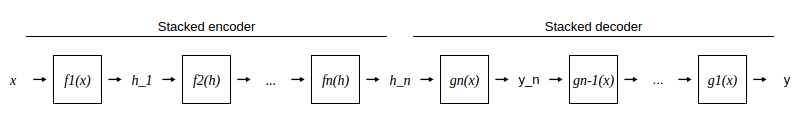
\includegraphics[width=\textwidth,height=\textheight,keepaspectratio]{sae.png}
  \caption{Stacked autoencoder.}
  \label{fig:sae}
\end{figure}

In subsection \ref{ch:dcae} we discuss techniques specifically useful in computer vision.
That includes application of convolutional layers and mixing training data with random noise
Subsection \ref{ch:sae} describes possible modifications of the learning objective.


\subsection{Autoencoders and computer vision}\label{ch:dcae}

Selecting a suitable model for computer vision task can be a tedious process.
Input data is often highly dimensional and contains hundreds of thousands of features for each input \ref{ILSVRC15}.
Model has to be flexible enough to address the issue of highly nonlinear relation between input features.
At the same time it has to be highly invariant to position of visual features, spatial transformations and noisy data.
All of this requirements lead to increased of model complexity.

In this subsection we discuss the means of increasing generalization properties of complex computer vision models and modification, more specific to autoencoders.

\subsubsection{Denoising autoencoders}

Learning high capacity models is prone to overfitting.
One of the common ways to decrease overfitting and make model learn useful features without actually changing the model is learning on a larger training corpus.

Denoising autoencoder approach \ref{Vincent2010} allows to increase variation in training data by adding random noise to images. We construct input examples by adding random noise to the dataset according to some parameter $alpha$: $\hat{x}=noise(x, \alpha)$.
Denoising autoencoder is yet supposed to reconstruct  the original image $L(x, g(f(\hat{x})))$.
This approach expects encoded representation to be stable and robust under condition of input corruption.
It also expects that denoising tasks would result in learning useful structure of input distribution.
Denoising autoencoders are reported to allow better generalization, when encoded features are provided to another model to perform classification task.

\subsubsection{Convolutional autoencoders}

One of the issues commonly encountered in computer vision tasks is spatial correlation of the data.
Neighboring pixels of a single image are rarely fully independent.
Fully-connected networks are ill-fitted for addressing such local correlation of data.
Furthermore, high dimensionality of computer vision data results in over-parametrization of such models and leads to overfitting.
Recent trends are clearly skewed towards convolutional models \cite{He2015, Szegedy2016}.
Convolutional models are consistently showing best results in computer vision competitions \cite{ILSVRC15, Zhou2016}.

Convolutional and maxpooling layers provide means of dimensionality reduction.
As described in section \ref{ch:cnn}, applying strided convolutions or pooling layers leads to decrease in resolution of the feature map.
Therefore convolutional and maxpooling layers are natural candidates for feature extraction in encoder network.

Convolutional networks depend on relatively small number of parameters.
This quality is desirable for learning useful feature mapping since it allows to avoid overfitting and, as a result, learning of identity mapping by the network.
As described, number of parameters of convolutional layer depends only on kernel size and depth of the feature map.
Number of parameters required by pooling layers is relatively small if not zero and does not depend on the size of the input.

\subsubsection{Deconvolutional layers and input reconstruction}

While convolutional layers are natural for feature extraction in encoder, reconstruction of highly dimensional input requires a different technique.
One approach is to use an inverse-like operation to convolution.
Deconvolution layer, also known as transposed convolution, is one possible approach.

Deconvolutional layers \cite{Zeiler2010} take as an input an image $y$ composed of $K_0$ color channels $y_1, ... , y_{K_0}$.
As a result of deconvolution process we would like obtain $K_1$ feature maps of the same image.
We can represent each cahnnel $c$ of $K_0$ channels as $K_1$ channels convolved with feature maps $f_{k,c}$:

\begin{equation}\label{eq:de}
  \sum^{K_1}_{k=1}=z^i_k \cdot f_{k,c} = y^i_{k,c}
\end{equation}

where $\cdot$ is a dot product.

Using this equation we would like to find latent feature maps $f_{k,c}$.
Since equation \ref{eq:de} is an under-determined and allows multiple solution.
Therefore a regularization term $z^i_k$ is added to encourage sparsity of the solutions.
With sparsity term we can express the cost function $C$ for input $y_i$:

\begin{equation}\label{eq:dec}
    C(y_i) = \frac{\lambda}{2} \sum^{K_o}_{c=1} ||\sum^{K_1}_{k=1}{z^i_k \cdot f_{k,c} - y^i_{k,c}}||^2_2 + \sum^{K_1}_{k=1}{|z^i_k|^p}
\end{equation}

where we assume mean square error as a reconstruction cost and $p$ as regularization norm.
Constant $\lambda$ balances contributions to the total cost between reconstruction and regularization terms.

Problem \ref{eq:dec} for simplicity can be decomposed into 2 sequential quadratic problems and solved using stochastic gradient descent method.

\subsubsection{Unpooling layers}

Like with convolutional layers, applying pooling layers results in change of shape of feature map.
In this subsection we describe a method that allows to effectively revert max-pooling layer preserving relative spatial position of extracted features as on original image.

As described in section \ref{ch:cnn} maxpooling layer with stride $k$.
Applying this layers allows to reduce size of feature map $k^2$ times while preserving arguable most important information about extracted features.
Max-pooling is crucial for convolutional neural networks for achieving position tolerance.

Inverse operation of max-pooling is not well defined, since maximum value must be placed somewhere inside original volume of size $k^2$. Naively, we can choose an index of a cell index inside projection volume and put maximum values uniformly into cells with that index.
This procedure is depicted on figure \ref{fig:pool}.
However, this approach destroes relative positioning of unpooled features.
In other words, pooling allows higher lever features to recognize a face by presence of a nose and a mouse within neighboring smaller regions, naive unpooling might place both this features into the same region on the image.

\begin{figure}[h!]
  \centering
    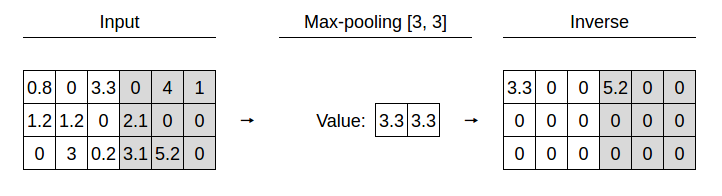
\includegraphics[width=\textwidth,height=\textheight,keepaspectratio]{pool.png}
  \caption{Pooling layer and naive inverse operation.}
  \label{fig:pool}
\end{figure}

To address this issue unpooling layer is introduced. Instead of using information about only maximum value of the feature in the region, unpooling layer also uses information about positioning of the feature. This positional information is called a mask. To every pooled value $x_{i,j}$ corresponds a single mask of size equal to pooling region size. To use mask information  unpooling layer take as an input volume with the same shape as produced by pooling layer. As follows, pooling layer describe in section \ref{ch:cnn} must also extract information about position of maximum value. This modification does not otherwise effect the layer nether during forward nor during backward pass. Application of unpooling layer is illustrated on figure \ref{fig:unpool}.

\begin{figure}[h!]
  \centering
    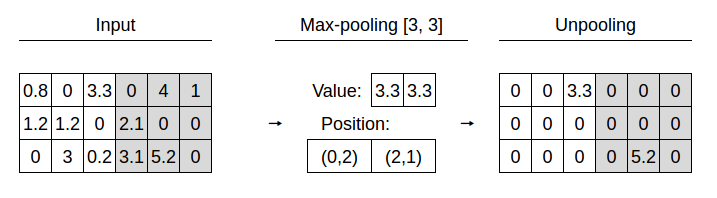
\includegraphics[width=\textwidth,height=\textheight,keepaspectratio]{unpool.png}
  \caption{Illustration of pooling and unpooling layers.}
  \label{fig:unpool}
\end{figure}

Unpooling layers contain no parameters and is not effected by backpropagation.

It worth noting, that mask information extracted by modified pooling layer depends on order of feature channels. As stated by the authors of the original algorithm, this might affect features, extracted by layers preceeding unpooling \cite{Zhao2015}.

\subsubsection{What-Where autoencoders}



\subsection{Extracting usefull features with Autoencoders}\label{ch:sae}

Standalone objective \ref{eq:ae} of autoencoder is not particularly useful.
In this section we are going to describe specific use-cases of applying autoencoders along with required modification of objective function.

\subsubsection{Sparse Autoencoders}\label{ch:vae}

Lets consider activations in the hidden layer $h$ for some input $x$:
\begin{equation}
  h(x) = \sigma(W_{h}x_{-1} + b_{h})
\end{equation}
where $W_h$ and $b_h$ are parameters of hidden layer $h$, $x_{-1}$ is output of the previous hidden layer and $\sigma$ is some activation function.
For example for sigmoid activation function every component of vector $h(x)$ would belong to interval $[0, 1]$.
Sparse autoencoders introduce additional term $l_{sparse}$ to loss function to add a constrain on the activations of the hidden layer $h$ \cite{Ng2011}:
\begin{equation}
  l_{total}(x) = l_{reconstruction}(x, g(f(x))) + \alpha*l_{sparse}(x, h(x))
\end{equation}
where $\alpha$ is a constant parameter.

Sparsity constrain tries to achieve low average activation $\hat{\rho}$ on the hidden layer:

\begin{equation}\label{eq:avgh}
  \rho = \sum_{i=1}^N h_i(x)/N
\end{equation}

For example, lets take a look at the case for sigmoid activation function in the hidden layer.
Sigmoid produces outputs in the interval $[0, 1]$. If we can guarantee average activation on the hidden layer $\hat{\rho} \leq 0.1$ we can rely upon the fact that no more than $10\%$ of hidden neurons would have activatoin close to $1.0$.

Sparse constrain allows to extract useful features even for relatively high number of hidden units. Specifically, decoder must be able to reconstruct original representation relying only on few high activation on the hidden layer.

There are several ways to enforce sparsity constrain.
It is possible to perform gradient descent directly for fixed value of $\hat{\rho}$ but we would have to perform a second pass over the dataset to calculate actual value of $\rho$. Instead we can simply nullify all but $k$ highest activation during the forward path through the network \cite{Kulkarni2015}.
Or apply negative log-likelyhood to the hidden layer of the network \cite{Zhao2015}.
At last, to achieve true zero values on the hidden layer we can use absolute value penalty $l_{sparce}=\sum_{i=1}^N |h_i|$ in conjunction with rectifier linear unit activation function \cite{Glorot2011}.

Sparse coding of the data has proven to be useful to solve classification problem.
In particular, for classification task requires us to assign one of $C$ exclusive classes we can train an autoencoder with $C$ hidden units. Once training converges we expect that features, learned by the hidden layer would somewhat correspond to classes of tasks. We can then use encoder part of the network as initialization of a classifier of the same architecture \cite{Masci2011}.
Such initialization leads to consistently better generalization results after supervised training of the classifier.

\subsubsection{Variational Autoencoders}\label{ch:vae}



% \subsection{Generative adcersarial nets}\label{ch:gan}
% \section{Autoencoders and feature interpretability}

% !TEX root = ./thesis.tex

\chapter{Model}
\label{cha:mode}

% !TEX root = ./thesis.tex

\chapter{Evaluation}
\label{ch:eval}

\section{Evaluation dataset}
\subsection{Data collection}

Access to large ammount of training data is crucial for appying deep learning models.
Successes of deep learning on image recognition and segmentation tasks can be attributed to existance of large research datasets as ILSVRC and Places365 \cite{ILSVRC15, Zhou2016} containing millions of labeled images.
Machine translation, NLP tasks \cite{Karpathy2014, Kim2014} often rely on low-dimensional word embedding models.
Such models, as for example as word2vec or Glove \cite{Mikolov2013, pennington2014glove}, are trained on terabytes of textual data.
Deep reinforcement models might use existing gaming engines to generate required training data "on the go".
As, for example Google DeepMind team uses Atari 2D games to generate data for Q-learning \cite{Mnih2013}.

For the purpose of this research we collect visual data using ViZDoom AI research platform \cite{Kempka2016}.
ViZDoom is a Doom-based platform for reinforcement learning.
It provides access to raw visual data from Doom gaming engine.
Doom is a first-person shooter (FPS) computer game utilizing 3D graphics.
In context of our research ViZDoom platform allows automatic visual data generation and collection.

We created multiple Doom maps specifically for our task using Slade \cite{Slade3} software.
Created maps provide high diversity of textures for better discrimination between images, captured from different positions on the map.
Other reason for diverse structures on the map is to explicitly brake simmetry of the map.
Symmetric maps look alike from different player positions.
Such position tend to be encoded with the same values of sparce features.
This represents a difficulty for evaluation and comparison of quality of sparce features.

We record multiple movement trajectories on each map.
More specifically, we record 10000-60000 consequtive images of unstructured movement of the player on the map for training purposes.
In addition to that, we record movement along well defined structured trajectories as a "circle" or an "eight" for model evaluation and comparison of quality of extracted features.


\begin{figure}
\centering
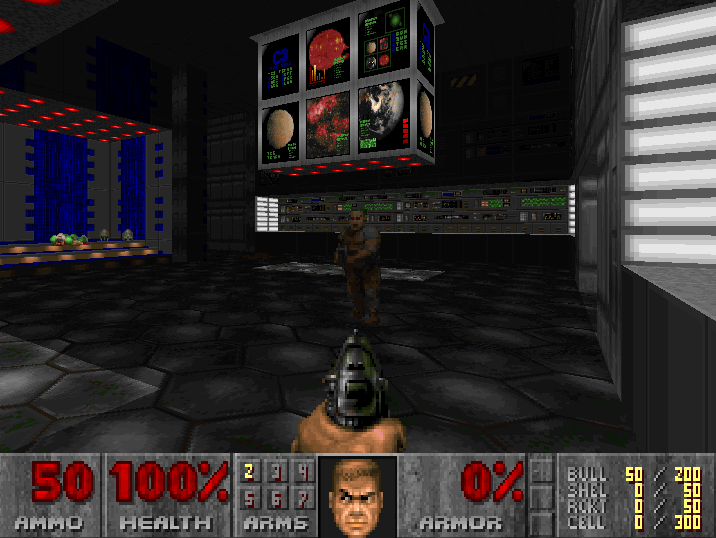
\includegraphics[width=.80\textwidth]{doom.png} %{CS0031}
\caption{Example of DoomII image collected with ViZDoom \cite{Kempka2016}.}
\label{fig:doom}
\end{figure}

\subsection{Dataset description}

Say few words about how your datasets look like and what trajectories you follow

\subsection{Data format}

Tell what is on the pictures

% !TEX root = ./thesis.tex

\chapter{Conclusion}
\label{ch:conc}



%Das geht dann so \cite{Lamport95}.


%%%----------------------------------------------------------
%%%Anhang
\appendix
% \include{anhang_a}	% Technische Ergänzungen
% \include{anhang_b}	% Inhalt der CD-ROM/DVD
% \include{anhang_c}	% Chronologische Liste der Änderungen
% \include{anhang_d}	% Quelltext dieses Dokuments

%%%----------------------------------------------------------
\MakeBibliography
%%%----------------------------------------------------------

%%%Messbox zur Druckkontrolle
\include{messbox}

\end{document}
